\section{Anforderungen und Nutzererwartungen}

\subsection{Produktbeschreibung}
\begin{figure}
  \centering
  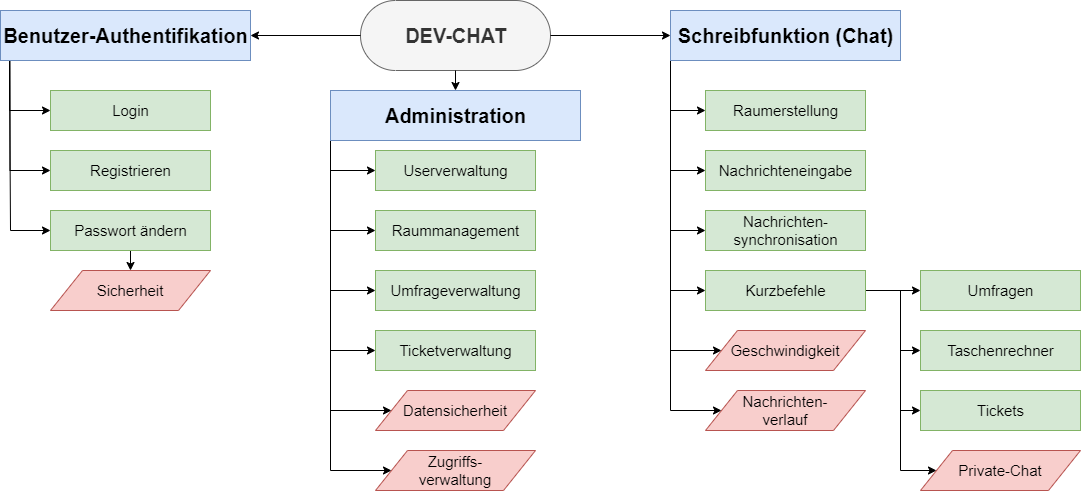
\includegraphics[width=1\textwidth, keepaspectratio]{images/Produktstruktur.png}
  \caption{Produktstruktur}
  \label{fig:Produktstruktur}
\end{figure}
Bei dem vorliegenden Produkt handelt es sich um eine Web-Messenger-Applikation namens \gqq{DEV-CHAT}, die es ermöglicht, mit anderen Nutzern zu chatten.
Die Abbilung~\ref{fig:Produktstruktur} stellt die Hauptfunktionen der Applikation dar.
Diese sind die Benutzer-Authentifikation, die Administration sowie die Schreibfunktion.
Ein Benutzer hat die Möglichkeit sich einen Account zu erstellen und sich mit diesem einzuloggen.
Damit ein User sich erfolgreich registrieren kann, müssen folgende Kritierien erfüllt werden:
\begin{itemize}
  \item Benutzername
  \begin{itemize}
    \item Der Benutzername muss mindestens 4 und maximal 16 Zeichen lang sein
    \item Der Benutzername darf nur aus lateinischen Buchstaben und Zahlen bestehen
    \item Der Benutzername \gqq{admin} in jeglicher Groß- und Kleinschreibung steht nicht für Benutzer zur Verfügung, auch nicht als Teilwort einer Namens
  \end{itemize}
  \item Passwort
  \begin{itemize}
    \item Das Passwort muss mindestens 8 lang sein
    \item Das Passwort muss mindestens einen Großbuchstaben, einen Kleinbuchstaben und eine Zahl enthalten
    \item Das Passwort darf nur aus lateinischen Buchstaben und Zahlen bestehen
  \end{itemize}
\end{itemize}  
Um die Sicherheit des Benutzerpassworts zu gewährleisten, wird dies bei der Registrierung mit einem Hashwert verschlüsselt und in einer Datenbank gespeichert.
Bei der Anmeldung wird der eingegebene Passwort-Hashwert mit dem in der Datenbank verglichen.
Ist dies erfolgreich, wird der Benutzer eingeloggt.
Ist dies nicht der Fall, wird der Benutzer benachrichtigt, dass die Anmeldedaten nicht korrekt sind. Zusätzlich bietet das Produkt die Möglichkeit, das Passwort zu ändern.
Hierfür muss der Benutzer sein aktuelles Passwort eingeben und ein neues Passwort eingeben, welches die gleichen Kritierien erfüllt.

\noindent
Neben der Benutzer-Authentifikation bietet das Produkt die Möglichkeit, einen Chatraum zu erstellen oder einem bestehenden beizutreten.
Bei der Erstellung eines Raumes, wird der \gqq{Raumname} aus drei englischen Wörtern zufällig generiert.
Dieser erhält ein Ablaufdatum, welches standardmäßig ein Tag ist.
In diesem Chatraum können Nachrichten mit anderen Personen ausgetauscht werden.
Zusätzlich findet bei dem anderen Chat eine Nachrichtensynchronisation statt.
Dies bedeutet, dass die Nachrichten, die in einem Chatraum geschrieben werden, auch in den anderen Chats angezeigt werden.
Hierbei findet kein Performance Verlust statt und das Senden sowie Sychronisieren einer Nachricht wirkt flüssig.
Ein Nachrichtenverlauf wird angezeigt, aufgrund dass alle Nachrichten einem Chatraum zugeordnet sind und diese in der Datenbank gespeichert werden.
Ein Benutzer hat die Möglichkeit Kurzbefehle innerhalb eines Chatraums zu verwenden.
Diese sind:
\begin{itemize}
  \item \gqq{/help} - Zeigt eine Liste mit allen Kurzbefehlen an
  \item \gqq{/survey} - Erstellt eine Umfrage mit den folgenden Parametern:
  \begin{itemize}
    \item Titel
    \item Beschreibung
    \item Antwortmöglichkeiten
    \item Zeitdauer
  \end{itemize}
  \item \gqq{/calc} - Bietet die Möglichkeit, eine einfache Rechnung durchzuführen
  \item \gqq{/whisper} - Sendet eine Nachricht an einen bestimmten Benutzer
  \item \gqq{/ticket} - Einsenden eines Fehlers
  \item \gqq{/vote} - Abstimmen einer Umfrage mit einer Antwortmöglichkeit mit dem folgenden Parameter:
  \begin{itemize}
    \item UmfrageID
    \item AntwortID
  \end{itemize}
\end{itemize}

\noindent
Die Administration ist zuständig für die Verwaltung der Benutzer und der Chat-Räume.
Die graphische Administrationsoberfläche kann nur der jeweilige Benutzer einsehen, der die Rolle \gqq{Admin} besitzt.
Der Admin ist hierbei zuständig für die Verwaltung von Benutzern, Räumen, Umfragen sowie Tickets.
Dieser kann Benutzer löschen, deren Passwort zurücksetzen oder dessen Berechtigungsstatus in \gqq{Standard} oder \gqq{Admin} ändern.
Er kann auch neue Chat-Räume mit einem Custom-Chat-Namen erstellen, löschen sowie das Ablaufsdatum eines Raumes ändern.
Zusätzlich kann dieser erstellte Umfragen löschen und das Ablaufdatum dieser ebenfalls umstellen.
Der Admin kann alle eingereichten Tickets einsehen und deren Status anpassen, falls diese bearbeitet wurden.
Die Tickets können in den Status \gqq{To Do}, oder \gqq{Done} geändert werden.

\subsection{Merkmale der Qualität}
\paragraph{Funktionalität}
%//TODO: @Johannes @Lukas - Bitte noch mal drüber schauen!
\begin{itemize}
  \item Benutzer-Authentifikation
  \begin{itemize}
    \item Benutzer registrieren
    \begin{itemize}
      \item Benutzername, Password, Confirm Password eingeben
      \newline 
      => Müssen die Kriterien erfüllen
    \end{itemize}
    \item Benutzer löschen
    \newline
    => Alle zugehörigen Daten (Chat Nachrichten, Umfragen etc.) werden gelöscht
    \item Benutzer anmelden
    \newline
    => Benutzername und Passwort eingeben
    \item Benutzer abmelden
    \newline
    => Benutzer wird ausgeloggt
    \item Benutzer Passwort ändern
    \begin{itemize}
      \item Altes und neues Passwort eingeben
      \newline
      => Das neue Passwort muss die Kriterien erfüllen
    \end{itemize}
  \end{itemize}
  \item Schreibfunktion (Chat)
    \begin{itemize}
      \item Chat-Raum erstellen
      \newline
      => Der Raumname wird aus drei englischen Wörtern zufällig generiert und man wird nach der Erstellung direkt in den Chat weitergeleitet
      \item Chat-Raum beitreten
      \newline
      => Beitreten des gewünschten Chat-Raums
      \item Nachrichten senden
      \newline
      => Nachrichten können in den aktuellen Chat-Raum gesendet werden
      \item Nachrichten empfangen
      \newline
      => Alle Benutzer im aktuellen Chat-Raum können Nachrichten synchron empfangen
      \item Nachrichtenverlauf anzeigen
      \newline
      => Alle Nachrichten des aktuellen Chat-Raums werden angezeigt
      \item Kurzbefehle verwenden
      \begin{itemize}
        \item \gqq{/help}
        \newline
        => Zeigt eine Liste mit allen Kurzbefehlen an
        \item \gqq{/survey}
        \newline
        => Erstellt eine Umfrage mit den folgenden Parametern:
        \begin{itemize}
          \item Titel
          \item Beschreibung
          \item Antwortmöglichkeiten
          \item Zeitdauer
        \end{itemize}
        \item \gqq{/calc} 
        \newline
        => Bietet die Möglichkeit, eine einfache Rechnung durchzuführen
        \item \gqq{/whisper} 
        \newline
        => Sendet eine Nachricht an einen bestimmten Benutzer
        \item \gqq{/ticket} 
        \newline
        => Einsenden eines Fehlers
        \item \gqq{/vote}
        \newline
        => Abstimmen einer Umfrage mit einer Antwortmöglichkeit mit dem folgenden Parameter:
        \begin{itemize}
          \item UmfrageID
          \item AntwortID
        \end{itemize}
    \end{itemize}
  \end{itemize}
  \item Administration
    \begin{itemize}
      \item Benutzer verwalten
      \begin{itemize}
        \item Benutzer anzeigen
        \newline
        => Alle Benutzer werden tabellarisch angezeigt
        \item Benutzer löschen
        \newline
        => Alle zugehörigen Daten (Chat Nachrichten, Umfragen, etc.)werden gelöscht
        \item Benutzer Passwort zurücksetzen
        \newline
        => Das Passwort wird auf den Namen des Benutzers zurückgesetzt
        \item Benutzer Berechtigungsstatus ändern
        \newline
        => Der Benutzer erhält die Rolle \gqq{Admin} oder \gqq{Standard}
      \end{itemize}
    \item Chat-Räume verwalten
      \begin{itemize}
        \item Chat-Räume anzeigen
        \newline
        => Alle Chat-Räume werden tabellarisch angezeigt
        \item Custom-Chat-Raum erstellen
        \newline
        => Es kann ein Custom-Chat-Raum mit einem gewünschten Namen erstellt werden
        \item Custom-Chat-Raum löschen
        \newline
        => Es können Chat-Räume gelöscht werden
        \item Ablaufdatum eins Chat-Raums ändern
        \newline
        => Es kann das Ablaufdatum eines Chat-Raums geändert werden
      \end{itemize}
    \item Umfragen verwalten
      \begin{itemize}
        \item Umfragen anzeigen
        \newline
        => Alle Umfragen werden tabellarisch angezeigt
        \item Umfragen löschen
        \newline
        => Es können Umfragen gelöscht werden
        \item Ablaufdatum einer Umfrage ändern
        \newline
        => Es kann das Ablaufdatum einer Umfrage geändert werden
      \end{itemize}
    \item Tickets verwalten
      \begin{itemize}
        \item Tickets anzeigen
        \newline
        => Alle Tickets werden tabellarisch angezeigt
        \item Tickets löschen
        \newline
        => Es können Tickets gelöscht werden
        \item Tickets bearbeiten
        \newline
        => Es kann der Status eines Tickets geändert werden
      \end{itemize}  
    \end{itemize}   
\end{itemize}

\paragraph{Effizienz}\mbox{} \\
\noindent
Die Web-Applikation agiert bei allen Benutzerinteraktionen schnell. Die Anwendung enthält keine Verzögerungen, die durch die Verarbeitung von Daten entstehen. Durch die Synchronisation der Chat-Räume bei allen Benutzern, wird die Performance nicht beeinträchtigt.

\paragraph{Kompatabilität}\mbox{} \\
\noindent
Die Web-Applikation ist kompatibel mit allen gängigen Browsern.
Die Applikation wurde mit den Browsern \gqq{Google Chrome}, \gqq{Mozilla Firefox} und \gqq{Microsoft Edge} getestet.
Die Applikation ist auch auf mobilen Endgeräten nutzbar.

\paragraph{Benutzbarkeit}\mbox{} \\
\noindent
Die Web-Applikation ist einfach zu bedienen. 
Die Benutzeroberfläche ist intuitiv und die Navigation ist selbsterklärend.
Die Applikation ist für alle Benutzer geeignet.
Die Applikation ist auch für Benutzer mit eingeschränkten Fähigkeiten geeignet.
Bei der Registrierung werden mithilfe der visuellen Kriterien bestimmte Fehlbedienungen verhindert.
Durch den Titel \gqq{Dev-Chat} wird schnell erkennbar, dass es sich um eine Applikation fürs Chatten handelt.
Diese ist aber hierbei für Entwickler spezifiziert.

\paragraph{Zuverlässigkeit}\mbox{} \\
\noindent
%//TODO: Zuverlässigkeit Text schreiben
KEIN PLAN WAS ICH HIER SCHREIBEN SOLL???

\paragraph{Sicherheit}\mbox{} \\
\noindent
Bei der Registrierung eines Benutzers wird das Passwort in der Datenbank mit einem Hashwert verschlüsselt.
Dieses wird anschließend bei der Anmeldung mit diesem wieder entschlüsselt.
Stimmt das eingebene Passwort mit dem entschlüsselten Passwort der Datenbank überein, dann wird der Benutzer angemeldet.
Während des Erstellungsprozesses erhält der Anwender die Berechtigung \gqq{Standard}.
Durch diese Berechtigung wird verhindert, dass die Benutzung der Administrationsoberfläche verwährt wird.
\newline
\newline
Die Sicherheit der Daten wird zustäzlich gewährleistet, indem im Backend des Systems dazu weitere Sicherheitsabfragen stattfinden, sodass das Manipulieren der Daten nutzlos ist.
Damit werden wie unter anderem die folgenden Angriffe verhindert:
\begin{itemize}
  \item SQL-Injection
  \item Cross-Site-Scripting
\end{itemize}

\paragraph{Wartbarkeit}\mbox{} \\
\noindent
 Die Applikation ist modular aufgebaut.
 Die einzelnen Komponenten sind in einzelne Klassen und einzelne Dateien aufgeteilt.
 Zugehörige Klassen wurden in einer Ordnerstruktur verpackt.
 Hierbei wurde darauf geachtet, dass das Frontend und Backend getrennt voneinander sind.
 Aufgrund des modularen Aufbaus können zusätzliches Features entwickelt und jegliche Konflikte implementiert werden. %TODO: Das noch mit den Kurzbefehlen ergänzen (das weiß glaub Johannes noch wie das perfekt geht)
Durch die Struktur der Anwendung ist es möglich, diese ohne großen Aufwand zu testen.

\paragraph{Übertragbarkeit}\mbox{} \\
\noindent
Die Web-Applikation ist unabhängig von dem Betriebsystem.
Diese ist in allen gängigen Browsern sowie auf mobilen Endgeräten nutzbar.
Hierbei wurde darauf geachtet, dass die Anwendung die Benutzerfreundlichkeit auf einem mobilen Endgerät nicht beeinträchtigt.

%TODO: Eigentlich gibt es noch im Bezug Quality of Use "Risikifreiheit" aber das ist ja eigentlich genau das gleich wie Sicherheit? Oder? 
%TODO: Verwendbarkeit 

\newpage
\subsection{Nutzererwartungen, Akzeptanzkriterien und dessen verschiedenen Nutzer}
Die Nutzererwartungen lassen sich in drei Kategorien unterteilen.
%//TODO @Phillipp: Du erwähnst nur Nutzererwartungen gehst aber nicht auf die Akzeptanzkriterien ein. Allgemein müsste hier ein einleitender Absatz hin.
%//TODO @Phillipp: Wahrscheinlich sind die folgenden Punkte eher paragraphs und nur die zwei nutzer subsubsections
\subsubsection{Verborgene Erwartungen}
Verborgene Erwartungen sind unbewusst und entstehen durch die Erfahrungen, die der Nutzer mit anderen Produkten gemacht hat.
Hierbei können dies bestimmte Interaktionen, Navigationen, Layouts und Designs sein.
Somit wird bei den meisten Applikationen erwartet, dass ein Fenster üblicherweise an der oberen rechten Seite mit einem Button geschlossen werden kann.
Bei einer Neuentwicklung einer Anwendung, dann sollte diese auf den gängisten Betriebssystemen/Browser lauffähig sein. 
\subsubsection{Prägende Erwartungen}
Prägende Erwartungen ergeben sich aus der Erfahrungen mit der Benutzung bestimmter Applikationen.
Einzelne Aspekte von Websites sind hierbei bekannt und die Benutzung ist intuitiv.
Ein Beispiel hierfür ist Social Media.
Die meisten Nutzer sind mit der Benutzung von Social Media Plattformen vertraut und kennen den Sinn und Zweck dieser Interaktionselemente.
Bei der Entwicklung einer neuen Anwendung, wird somit erwartet, dass diese Elemente vorhanden sind.
\subsubsection{Aktuelle Erwartungen}
Aktuelle Erwartungen sind bewusste Erfahrung und sind mit der aktuellen Situation verbunden.
Nutzer sind bewusst auf einer Website und wissen was sie dort finden möchten.
%//TODO @Phillipp: Seitenzahl einfügen
Wenn einer dieser Erwartungen nicht erfüllt wird, ist die natürliche Nutzerreaktion, das Verlassen dieser Website \autocite[vgl.][S. ]{noauthor_user_nodate}.

\subsubsection{Akzeptanzkriterien}
Akzeptanzkriterien beschreiben, wann eine bestimmte Anforderung in einem Entwicklungsteam als abgeschlossen gelten kann.
Hierbei ist zu beachten, dass diese objektiv und eindeutig zu überprüfen sind, damit alle Erwartungen wie gewollt umgesetzt worden sind. \autocite[vgl.][S. ]{noauthor_akzeptanzkriterien_nodate}

\subsubsection{Technisch wenig versierter Nutzer}
Ein technischer wenig versierter Nutzer ist ein Nutzer, der nicht über die nötigen Kenntnisse verfügt, um eine Anwendung intuitiv zu bedienen.
Dieser könnte hierbei sich einen Account erstellen, einloggen und die Chat-Räume erstellen/betreten.
Diesem Nutzer wäre aber nicht bewusst, dass ein Chat-Raum Kurzbefehle zur Verfügung hat.
Zusätzlich würde er auch sich nicht auseinandersetzen, wie er diese nutzen kann.
Das Design der Anwendung ist für ihn unerträglich und er würde sich nicht lange mit der Anwendung beschäftigen.
Falls dieser Benutzer jedoch bewusst eine Anleitung zur Verfügung hat, würde er sich mit der Anwendung auseinandersetzen und diese nutzen.
Besitzt der Anwender Admin-Rechte, dann könnte dies ein kritisches Problem darstellen, da dieser die Chat-Räume, Benutzer, Umfragen löschen könnte, ohne dass dieser dies bewusst ist.
Zusätzlich werden Berechtigungen anderer Benutzer geändert und dieser könnte plötzlich Admin-Rechte besitzen.

\subsubsection{Technische versierter Nutzer}
Bei einem technisch versierten Nutzer hingegen, liegen die Erwartungen gegenteilig zu der anderen Benutzergruppe.
Dieser besitzt bereits Erfahrungen mit der Benutzung von Chat-Programmen und ist somit mit den Funktionen vertraut.
Dieser erwartet eine einfache und intuitive Bedienung, sowie eine schnelle Reaktion der Web-Applikation.
Da ein Chat-Fenster einem Terminal ähnlich ist, wird der Nutzer auch hier erwarten, dass er bestimmte Befehle eingeben kann, um bestimmte Funktionen auszulösen.
Wenn diese Benutzergruppe einer der Kurzbefehle nicht kennt oder nicht weiß, wie diese funktionieren, wird er sicherlich testen, ob er mit dem Befehl /help nützliche Informationen herausfinden kann.
Wenn er hierbei immernoch ein Problem besteht, wird dieser sich Dokumentation der Applikation anschauen oder sich an den Admin wenden.
Falls dieser Nutzer selbst ein Admin ist, wird er sich mit der Administrationsoberfläche vertraut machen und diese nur für notwendige Änderungen nutzen.

\subsection{Spezifizieren einer Anforderungen in „halbformaler“ Beschreibung}
\begin{table}[h!]
  \centering
  \resizebox{\columnwidth}{!}{%
  \begin{tabular}{l|l}
  Beschreibung  & Anforderung                                          \\ \hline
  Funktion      & Benutzer registrieren                                \\ \hline
  Beschreibung  & Einen neuen Benutzer für den "DEV-Chat" registrieren \\ \hline
  Eingaben &
    \begin{tabular}[c]{@{}l@{}}Benutzerdaten:\\ Benutzername, 2x Passwort (Das 2te Passwort für die Bestätigung)\end{tabular} \\ \hline
  Ausgaben      & -                                                    \\ \hline
  Abfolge &
    \begin{tabular}[c]{@{}l@{}}Nutzer öffnet die Web-Applikation "Dev-Chat"\\ Klicken des Hyperlinks "create Account"\\ Benutzername eingeben\\ Passwort eingeben\\ Confirm Passwort eingeben\\ Klicken des Buttons "Create"\end{tabular} \\ \hline
  Ausnahmen     & Benutzername existiert bereits                       \\ \hline
  Vorbedingung  & -                                                    \\ \hline
  Nachbedingung & Benutzer wird nach der Erstellung direkt eingeloggt  \\ \hline
  Einschränkung &
    \begin{tabular}[c]{@{}l@{}}Benutzername entspricht nicht den Richtlinien\\ Passwort entspricht nicht den Richtlinien\\ Confirm Passwort stimmt nicht mit dem Passwort überein\end{tabular}
  \end{tabular}%
  }
\end{table}